\documentclass[]{article}
\usepackage{lmodern}
\usepackage{amssymb,amsmath}
\usepackage{ifxetex,ifluatex}
\usepackage{fixltx2e} % provides \textsubscript
\ifnum 0\ifxetex 1\fi\ifluatex 1\fi=0 % if pdftex
  \usepackage[T1]{fontenc}
  \usepackage[utf8]{inputenc}
\else % if luatex or xelatex
  \ifxetex
    \usepackage{mathspec}
  \else
    \usepackage{fontspec}
  \fi
  \defaultfontfeatures{Ligatures=TeX,Scale=MatchLowercase}
\fi
% use upquote if available, for straight quotes in verbatim environments
\IfFileExists{upquote.sty}{\usepackage{upquote}}{}
% use microtype if available
\IfFileExists{microtype.sty}{%
\usepackage{microtype}
\UseMicrotypeSet[protrusion]{basicmath} % disable protrusion for tt fonts
}{}
\usepackage[margin=1in]{geometry}
\usepackage{hyperref}
\hypersetup{unicode=true,
            pdftitle={Considerações sobre o impacto do valor do desvio-padrão},
            pdfauthor={Luiz Fernando Palin Droubi},
            pdfborder={0 0 0},
            breaklinks=true}
\urlstyle{same}  % don't use monospace font for urls
\usepackage{graphicx,grffile}
\makeatletter
\def\maxwidth{\ifdim\Gin@nat@width>\linewidth\linewidth\else\Gin@nat@width\fi}
\def\maxheight{\ifdim\Gin@nat@height>\textheight\textheight\else\Gin@nat@height\fi}
\makeatother
% Scale images if necessary, so that they will not overflow the page
% margins by default, and it is still possible to overwrite the defaults
% using explicit options in \includegraphics[width, height, ...]{}
\setkeys{Gin}{width=\maxwidth,height=\maxheight,keepaspectratio}
\IfFileExists{parskip.sty}{%
\usepackage{parskip}
}{% else
\setlength{\parindent}{0pt}
\setlength{\parskip}{6pt plus 2pt minus 1pt}
}
\setlength{\emergencystretch}{3em}  % prevent overfull lines
\providecommand{\tightlist}{%
  \setlength{\itemsep}{0pt}\setlength{\parskip}{0pt}}
\setcounter{secnumdepth}{5}
% Redefines (sub)paragraphs to behave more like sections
\ifx\paragraph\undefined\else
\let\oldparagraph\paragraph
\renewcommand{\paragraph}[1]{\oldparagraph{#1}\mbox{}}
\fi
\ifx\subparagraph\undefined\else
\let\oldsubparagraph\subparagraph
\renewcommand{\subparagraph}[1]{\oldsubparagraph{#1}\mbox{}}
\fi

%%% Use protect on footnotes to avoid problems with footnotes in titles
\let\rmarkdownfootnote\footnote%
\def\footnote{\protect\rmarkdownfootnote}

%%% Change title format to be more compact
\usepackage{titling}

% Create subtitle command for use in maketitle
\newcommand{\subtitle}[1]{
  \posttitle{
    \begin{center}\large#1\end{center}
    }
}

\setlength{\droptitle}{-2em}

  \title{Considerações sobre o impacto do valor do desvio-padrão}
    \pretitle{\vspace{\droptitle}\centering\huge}
  \posttitle{\par}
  \subtitle{nas amostras de distribuição lognormal}
  \author{Luiz Fernando Palin Droubi}
    \preauthor{\centering\large\emph}
  \postauthor{\par}
      \predate{\centering\large\emph}
  \postdate{\par}
    \date{18 de outubro de 2018}


\begin{document}
\maketitle

\section{INTRODUÇÃO}\label{introducao}

Segundo Limpert (LIMPERT et al., 2001, p. 346), distribuições lognormais
de diversas ciências tem, em geral, valores de \(s^*\) variando de 1,1 a
33 (na escala natural, entre 0,095 e 3,497), sendo que o mais comum é
que estes valores estejam entre 1,4 e 3 (0,336 \(\leq s \leq\) 1,099).

Na Engenharia de Avaliações, temos:

\begin{itemize}
\tightlist
\item
  Hochheim (HOCHHEIM, 2015, p. 21): \(s^* =\) 1,851.
\end{itemize}

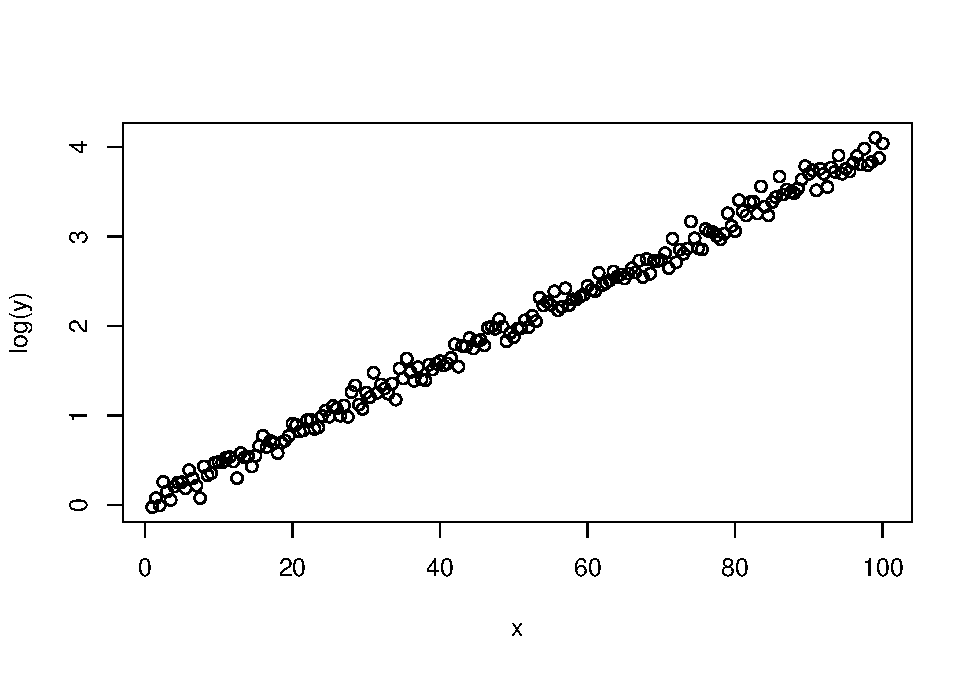
\includegraphics{Impacto_sigma_files/figure-latex/unnamed-chunk-2-1.pdf}

\section{EXEMPLOS DE APLICAÇÃO}\label{exemplos-de-aplicacao}

\subsection{EXEMPLO 1}\label{exemplo-1}

\subsubsection{\texorpdfstring{GERAÇÃO DE DADOS LOGNORMAIS COM
\(s^* = 1.1\)}{GERAÇÃO DE DADOS LOGNORMAIS COM s\^{}* = 1.1}}\label{geracao-de-dados-lognormais-com-s-1.1}

\subsubsection{GRÁFICOS}\label{graficos}

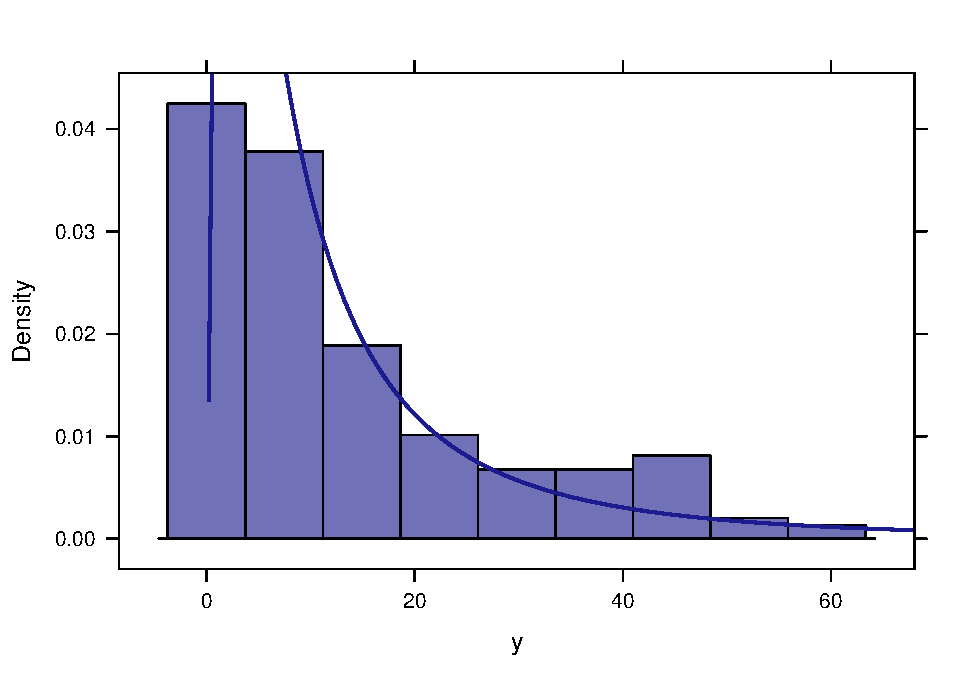
\includegraphics{Impacto_sigma_files/figure-latex/unnamed-chunk-4-1.pdf}

\subsection{EXEMPLO 2}\label{exemplo-2}

Mantido mesmo vetor x criado anteriormente.

\subsubsection{\texorpdfstring{GERAÇÃO DE DADOS LOGNORMAIS COM
\(s^* = 1,25\)}{GERAÇÃO DE DADOS LOGNORMAIS COM s\^{}* = 1,25}}\label{geracao-de-dados-lognormais-com-s-125}

\subsubsection{GRÁFICOS}\label{graficos-1}

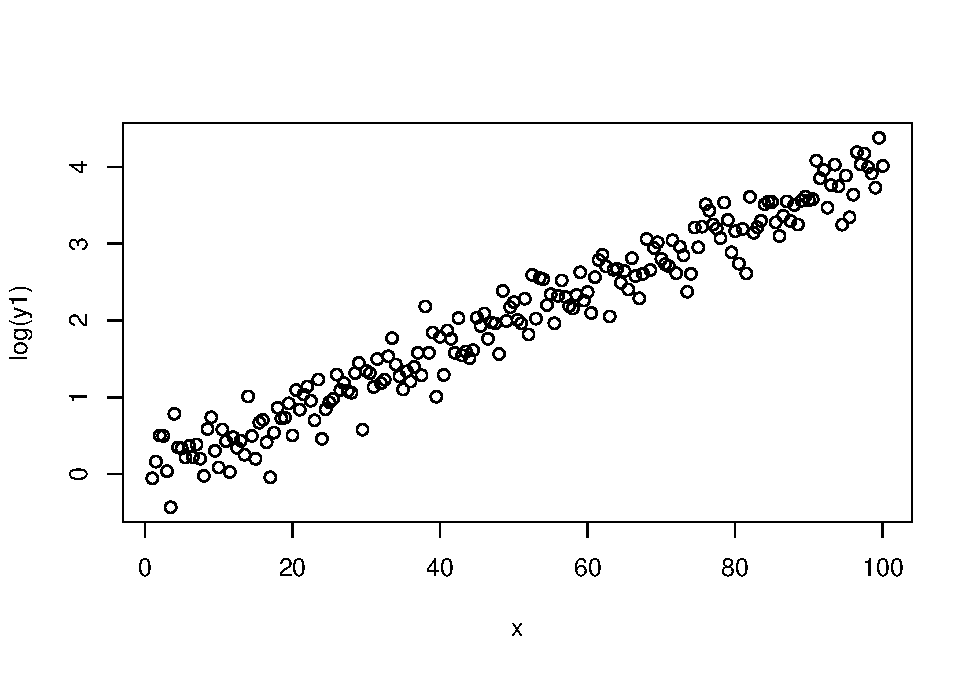
\includegraphics{Impacto_sigma_files/figure-latex/unnamed-chunk-7-1.pdf}

\subsection{EXEMPLO 3}\label{exemplo-3}

Mantido mesmo vetor x criado anteriormente.

\subsubsection{\texorpdfstring{GERAÇÃO DE DADOS LOGNORMAIS COM
\(s^* = 1,5\)}{GERAÇÃO DE DADOS LOGNORMAIS COM s\^{}* = 1,5}}\label{geracao-de-dados-lognormais-com-s-15}

\subsubsection{GRÁFICOS}\label{graficos-2}

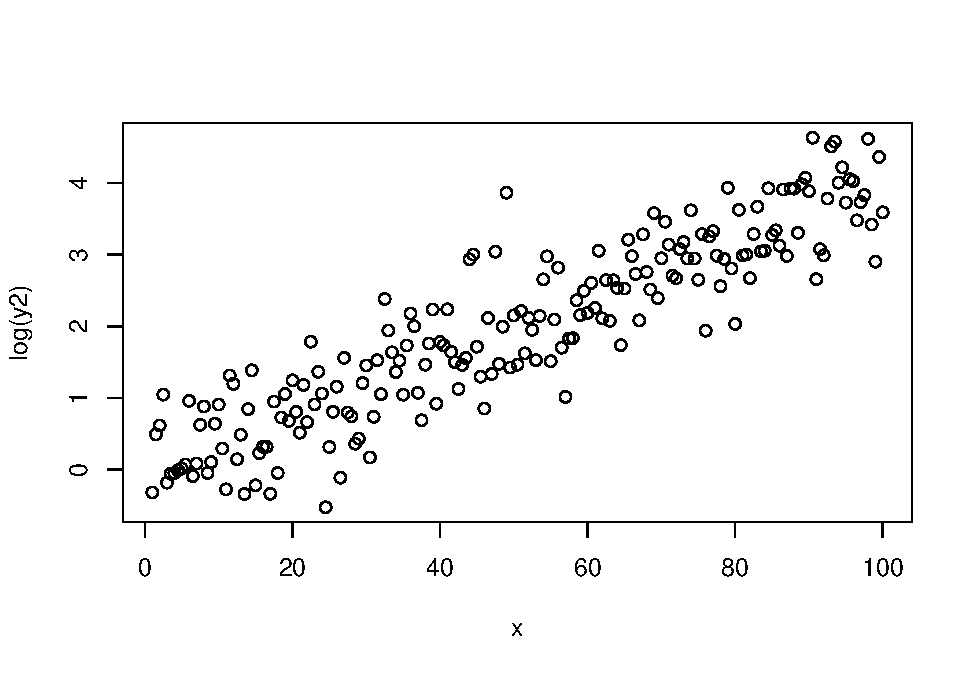
\includegraphics{Impacto_sigma_files/figure-latex/unnamed-chunk-10-1.pdf}

\subsection{EXEMPLO 4}\label{exemplo-4}

Mantido mesmo vetor x criado anteriormente.

\subsubsection{\texorpdfstring{GERAÇÃO DE DADOS LOGNORMAIS COM
\(s^* = 2\)}{GERAÇÃO DE DADOS LOGNORMAIS COM s\^{}* = 2}}\label{geracao-de-dados-lognormais-com-s-2}

\subsubsection{GRÁFICOS}\label{graficos-3}

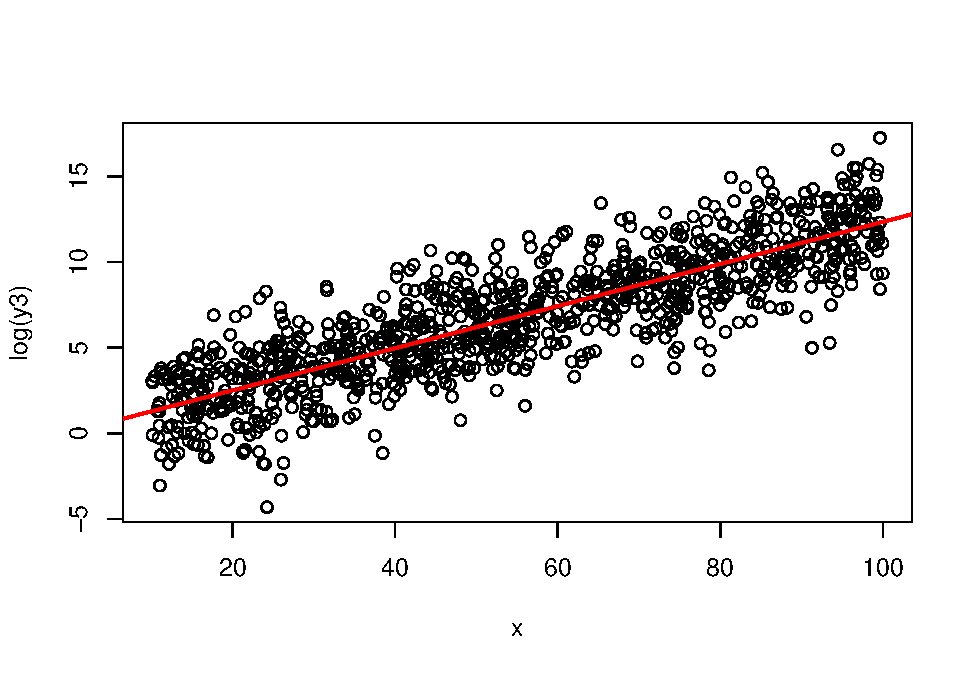
\includegraphics{Impacto_sigma_files/figure-latex/unnamed-chunk-13-1.pdf}

\subsection{EXEMPLO 5}\label{exemplo-5}

Mantido mesmo vetor x criado anteriormente.

\subsubsection{\texorpdfstring{GERAÇÃO DE DADOS LOGNORMAIS COM
\(s^* = 3\)}{GERAÇÃO DE DADOS LOGNORMAIS COM s\^{}* = 3}}\label{geracao-de-dados-lognormais-com-s-3}

\subsubsection{GRÁFICOS}\label{graficos-4}

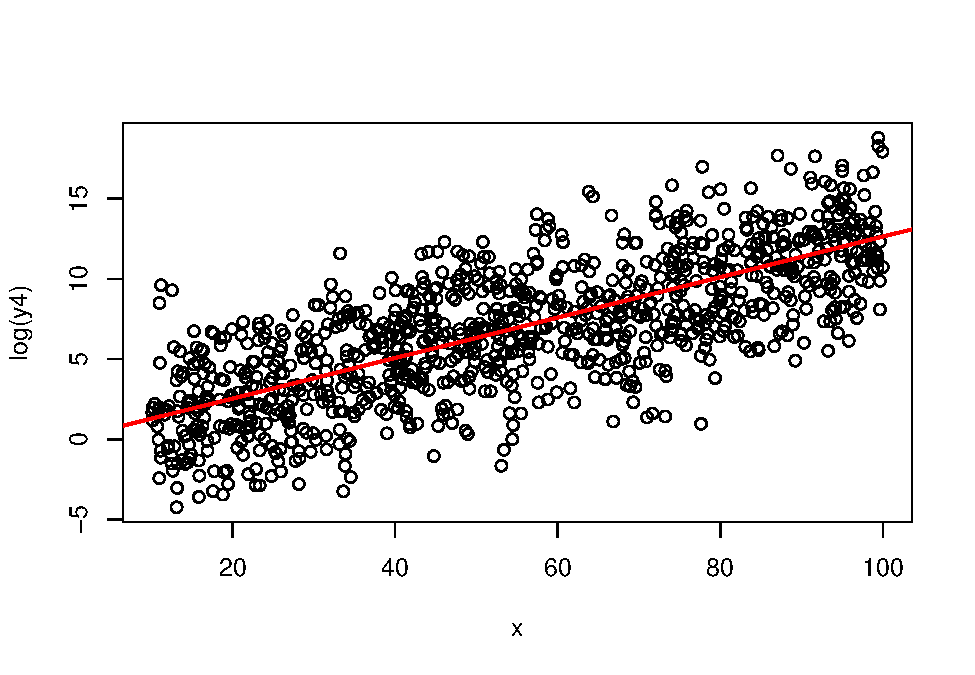
\includegraphics{Impacto_sigma_files/figure-latex/unnamed-chunk-16-1.pdf}

\subsection{MODELOS}\label{modelos}

\begin{table}[!htbp] \centering 
  \caption{} 
  \label{} 
\begin{tabular}{@{\extracolsep{5pt}}lccccc} 
\\[-1.8ex]\hline 
\hline \\[-1.8ex] 
 & \multicolumn{5}{c}{\textit{Dependent variable:}} \\ 
\cline{2-6} 
\\[-1.8ex] & log(y) & log(y1) & log(y2) & log(y3) & log(y4) \\ 
\\[-1.8ex] & (1) & (2) & (3) & (4) & (5)\\ 
\hline \\[-1.8ex] 
 x & 0.125$^{***}$ & 0.125$^{***}$ & 0.126$^{***}$ & 0.123$^{***}$ & 0.124$^{***}$ \\ 
  & (0.001) & (0.002) & (0.002) & (0.002) & (0.004) \\ 
  & & & & & \\ 
 Constant & $-$0.041 & $-$0.026 & 0.019 & 0.050 & $-$0.015 \\ 
  & (0.084) & (0.098) & (0.116) & (0.148) & (0.217) \\ 
  & & & & & \\ 
\hline \\[-1.8ex] 
Observations & 1,000 & 1,000 & 1,000 & 1,000 & 1,000 \\ 
R$^{2}$ & 0.891 & 0.859 & 0.814 & 0.720 & 0.548 \\ 
Adjusted R$^{2}$ & 0.891 & 0.859 & 0.813 & 0.720 & 0.548 \\ 
Residual Std. Error (df = 998) & 1.137 & 1.318 & 1.568 & 1.991 & 2.922 \\ 
F Statistic (df = 1; 998) & 8,162.732$^{***}$ & 6,078.971$^{***}$ & 4,357.517$^{***}$ & 2,565.384$^{***}$ & 1,212.096$^{***}$ \\ 
\hline 
\hline \\[-1.8ex] 
\textit{Note:}  & \multicolumn{5}{r}{$^{*}$p$<$0.1; $^{**}$p$<$0.05; $^{***}$p$<$0.01} \\ 
\end{tabular} 
\end{table}

\subsection{ESTIMATIVAS}\label{estimativas}

\subsubsection{Usando o primeiro modelo}\label{usando-o-primeiro-modelo}

\begin{enumerate}
\def\labelenumi{\alph{enumi}.}
\tightlist
\item
  Moda
\end{enumerate}

\begin{verbatim}
##        1 
## 138.1358
\end{verbatim}

\begin{enumerate}
\def\labelenumi{\alph{enumi}.}
\setcounter{enumi}{1}
\tightlist
\item
  Mediana
\end{enumerate}

\begin{verbatim}
##        1 
## 503.6085
\end{verbatim}

\begin{enumerate}
\def\labelenumi{\alph{enumi}.}
\setcounter{enumi}{2}
\tightlist
\item
  Média
\end{enumerate}

\begin{verbatim}
##        1 
## 961.5823
\end{verbatim}

\subsubsection{Usando o segundo modelo}\label{usando-o-segundo-modelo}

\begin{enumerate}
\def\labelenumi{\alph{enumi}.}
\tightlist
\item
  Moda
\end{enumerate}

\begin{verbatim}
##        1 
## 90.00315
\end{verbatim}

\begin{enumerate}
\def\labelenumi{\alph{enumi}.}
\setcounter{enumi}{1}
\tightlist
\item
  Mediana
\end{enumerate}

\begin{verbatim}
##        1 
## 510.8466
\end{verbatim}

\begin{enumerate}
\def\labelenumi{\alph{enumi}.}
\setcounter{enumi}{2}
\tightlist
\item
  Média
\end{enumerate}

\begin{verbatim}
##        1 
## 1217.046
\end{verbatim}

\subsubsection{Usando o terceiro modelo}\label{usando-o-terceiro-modelo}

\begin{enumerate}
\def\labelenumi{\alph{enumi}.}
\tightlist
\item
  Moda
\end{enumerate}

\begin{verbatim}
##        1 
## 47.88896
\end{verbatim}

\begin{enumerate}
\def\labelenumi{\alph{enumi}.}
\setcounter{enumi}{1}
\tightlist
\item
  Mediana
\end{enumerate}

\begin{verbatim}
##       1 
## 559.858
\end{verbatim}

\begin{enumerate}
\def\labelenumi{\alph{enumi}.}
\setcounter{enumi}{2}
\tightlist
\item
  Média
\end{enumerate}

\begin{verbatim}
##        1 
## 1914.252
\end{verbatim}

\subsubsection{Usando o quarto modelo}\label{usando-o-quarto-modelo}

\begin{enumerate}
\def\labelenumi{\alph{enumi}.}
\tightlist
\item
  Moda
\end{enumerate}

\begin{verbatim}
##        1 
## 9.313405
\end{verbatim}

\begin{enumerate}
\def\labelenumi{\alph{enumi}.}
\setcounter{enumi}{1}
\tightlist
\item
  Mediana
\end{enumerate}

\begin{verbatim}
##        1 
## 491.4793
\end{verbatim}

\begin{enumerate}
\def\labelenumi{\alph{enumi}.}
\setcounter{enumi}{2}
\tightlist
\item
  Média
\end{enumerate}

\begin{verbatim}
##        1 
## 3570.291
\end{verbatim}

\subsubsection{Usando o quinto modelo}\label{usando-o-quinto-modelo}

\begin{enumerate}
\def\labelenumi{\alph{enumi}.}
\tightlist
\item
  Moda
\end{enumerate}

\begin{verbatim}
##          1 
## 0.09514152
\end{verbatim}

\begin{enumerate}
\def\labelenumi{\alph{enumi}.}
\setcounter{enumi}{1}
\tightlist
\item
  Mediana
\end{enumerate}

\begin{verbatim}
##        1 
## 485.3153
\end{verbatim}

\begin{enumerate}
\def\labelenumi{\alph{enumi}.}
\setcounter{enumi}{2}
\tightlist
\item
  Média
\end{enumerate}

\begin{verbatim}
##        1 
## 34661.79
\end{verbatim}

\subsection{VISUALIZAÇÃO GRÁFICA}\label{visualizacao-grafica}

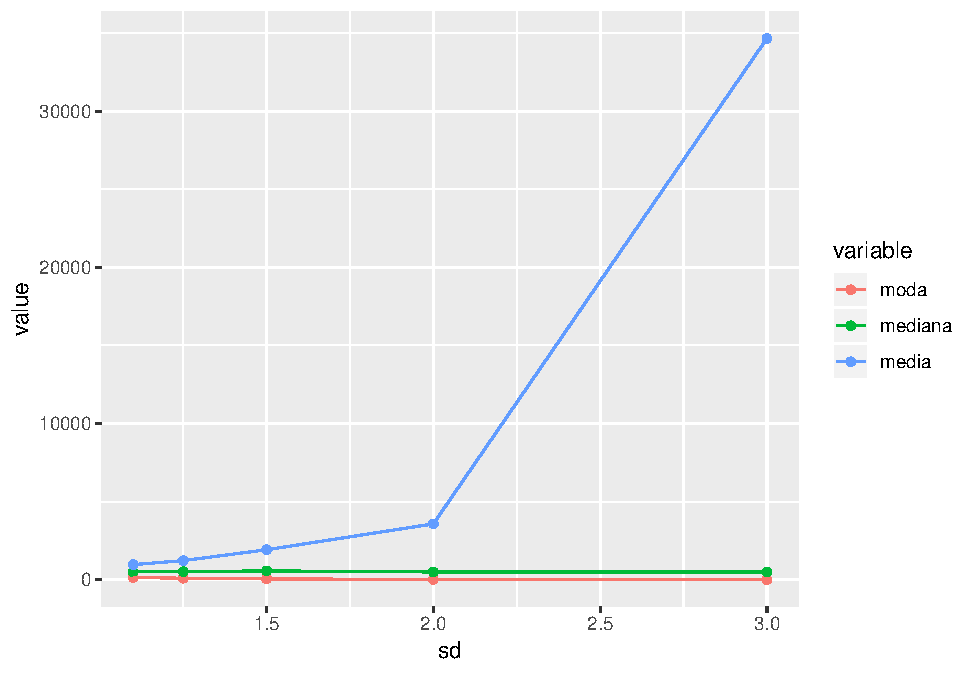
\includegraphics{Impacto_sigma_files/figure-latex/unnamed-chunk-36-1.pdf}

\subsection{VALIDAÇÃO CRUZADA}\label{validacao-cruzada}

\subsubsection{Modelo 1}\label{modelo-1}

\begin{verbatim}
## [1] 155510.7
\end{verbatim}

\begin{verbatim}
## [1] 138927.5
\end{verbatim}

\begin{verbatim}
## [1] 133838.6
\end{verbatim}

\subsubsection{Modelo 2}\label{modelo-2}

\begin{verbatim}
## [1] 196681
\end{verbatim}

\begin{verbatim}
## [1] 171146.3
\end{verbatim}

\begin{verbatim}
## [1] 160454.8
\end{verbatim}

\subsubsection{Modelo 3}\label{modelo-3}

\begin{verbatim}
## [1] 290597
\end{verbatim}

\begin{verbatim}
## [1] 272264.3
\end{verbatim}

\begin{verbatim}
## [1] 273938.6
\end{verbatim}

\subsubsection{Modelo 4}\label{modelo-4}

\begin{verbatim}
## [1] 1865827
\end{verbatim}

\begin{verbatim}
## [1] 1865774
\end{verbatim}

\begin{verbatim}
## [1] 1865451
\end{verbatim}

\subsubsection{Modelo 5}\label{modelo-5}

\begin{verbatim}
## [1] 9779082
\end{verbatim}

\begin{verbatim}
## [1] 9779023
\end{verbatim}

\begin{verbatim}
## [1] 9775666
\end{verbatim}

\subsubsection{VISUALIZAÇÂO VALIDAÇÃO
CRUZADA}\label{visualizacao-validacao-cruzada}

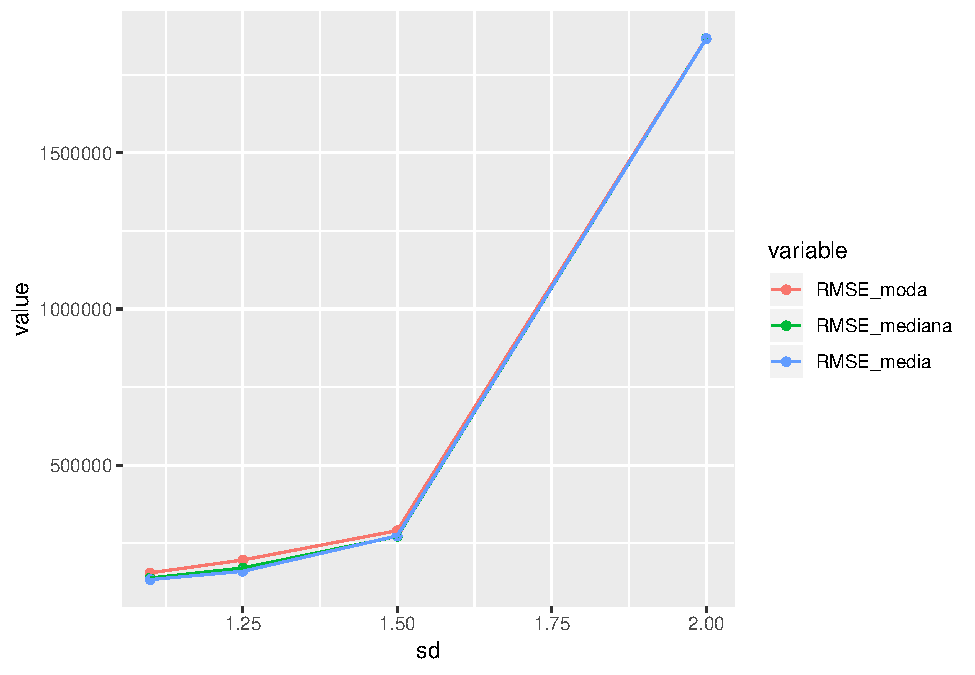
\includegraphics{Impacto_sigma_files/figure-latex/unnamed-chunk-43-1.pdf}

\section{REGRESSÃO À MEDIANA}\label{regressao-a-mediana}

\section{VALIDAÇÃO CRUZADA}\label{validacao-cruzada-1}

\subsection{Modelo 1}\label{modelo-1-1}

\begin{verbatim}
## [1] 43663.7
\end{verbatim}

\subsection{Modelo 2}\label{modelo-2-1}

\begin{verbatim}
## [1] 55736.13
\end{verbatim}

\subsection{Modelo 3}\label{modelo-3-1}

\begin{verbatim}
## [1] 61513.52
\end{verbatim}

\subsection{Modelo 4}\label{modelo-4-1}

\begin{verbatim}
## [1] 208947.1
\end{verbatim}

\subsection{Modelo 5}\label{modelo-5-1}

\begin{verbatim}
## [1] 1178752
\end{verbatim}

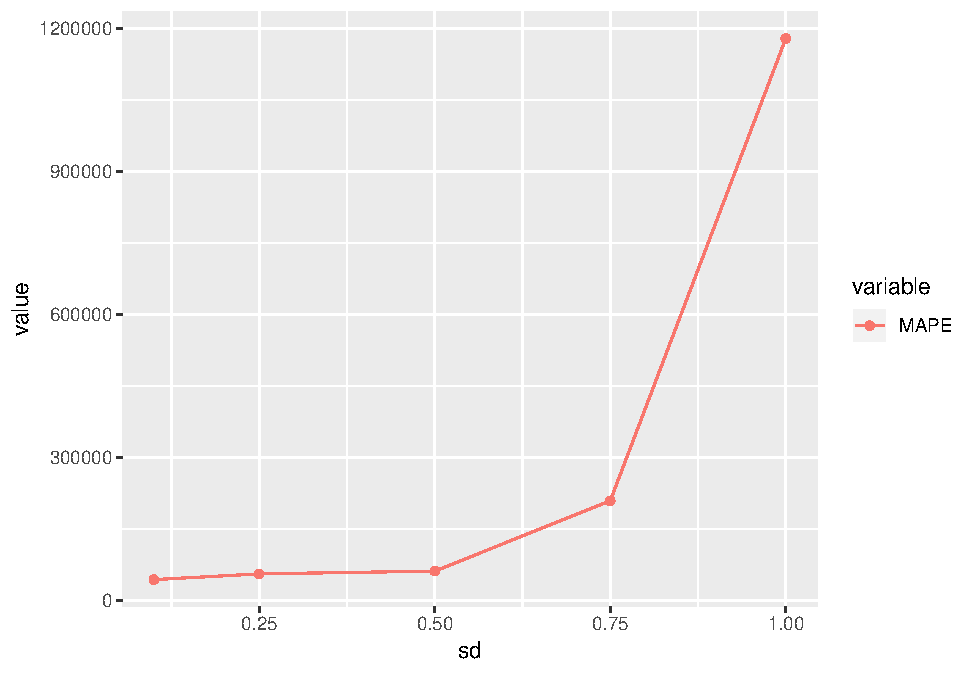
\includegraphics{Impacto_sigma_files/figure-latex/unnamed-chunk-50-1.pdf}

\section{SIMULAÇÕES DE MONTE CARLO}\label{simulacoes-de-monte-carlo}

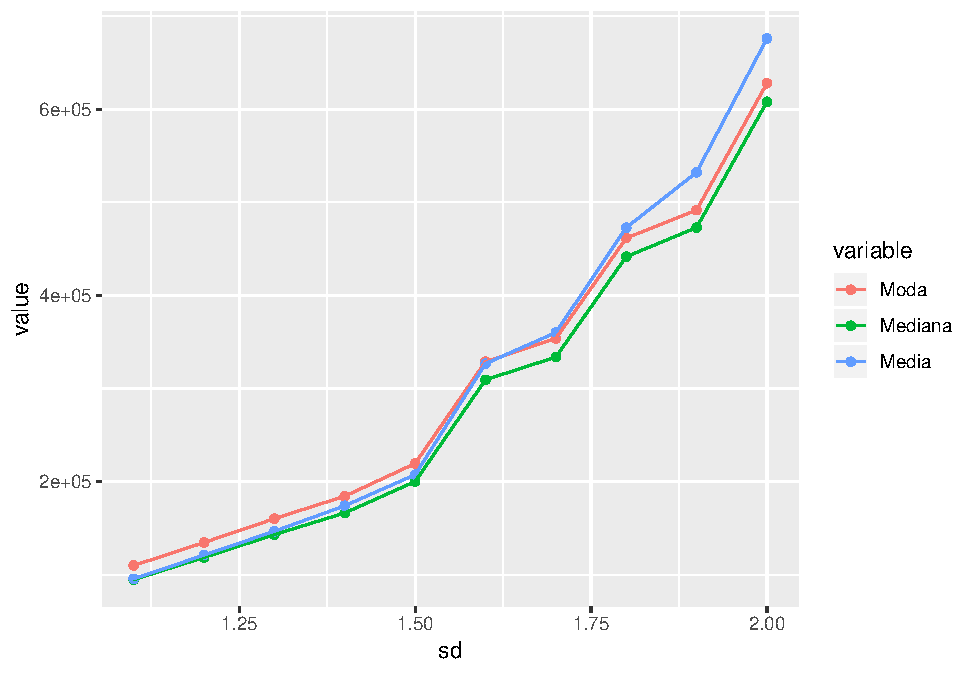
\includegraphics{Impacto_sigma_files/figure-latex/unnamed-chunk-53-1.pdf}
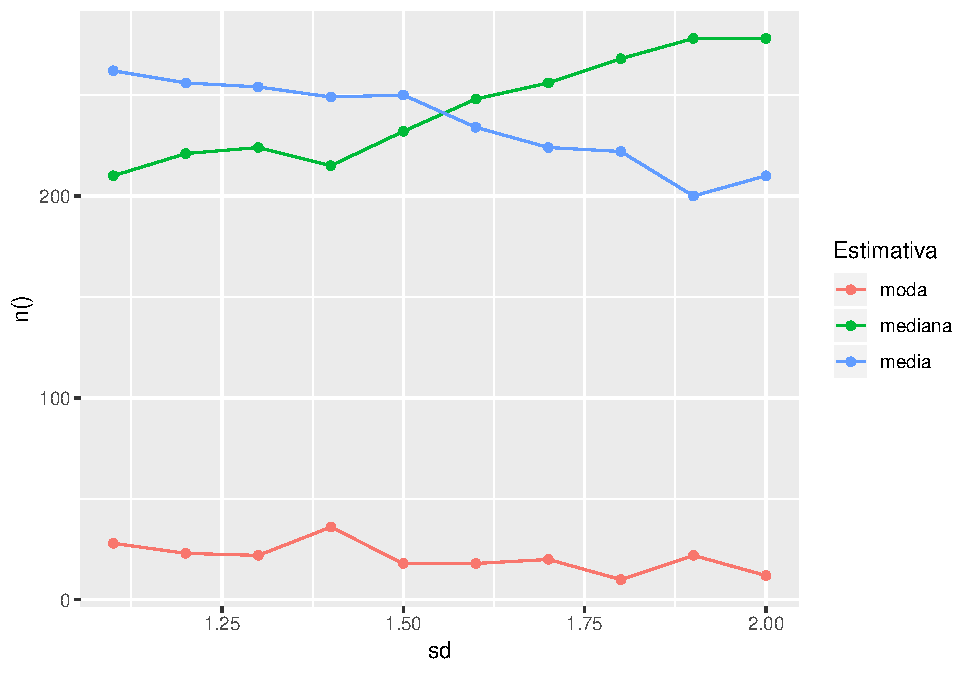
\includegraphics{Impacto_sigma_files/figure-latex/unnamed-chunk-54-1.pdf}

\section*{REFERÊNCIAS}\label{referencias}
\addcontentsline{toc}{section}{REFERÊNCIAS}

\hypertarget{refs}{}
\hypertarget{ref-hochheim}{}
HOCHHEIM, N. \textbf{Engenharia de avaliações - módulo básico}.
Florianópolis: IBAPE - SC, 2015.

\hypertarget{ref-limpert}{}
LIMPERT, E.; A. STAHEL, W.; ABBT, M. Log-normal distributions across the
sciences: Keys and clues., v. 51, p. 341, 2001.


\end{document}
